\section{Discussion}

\begin{figure}[t]
    \centering

    \begin{subfigure}[b]{0.49\textwidth}
    \centering
    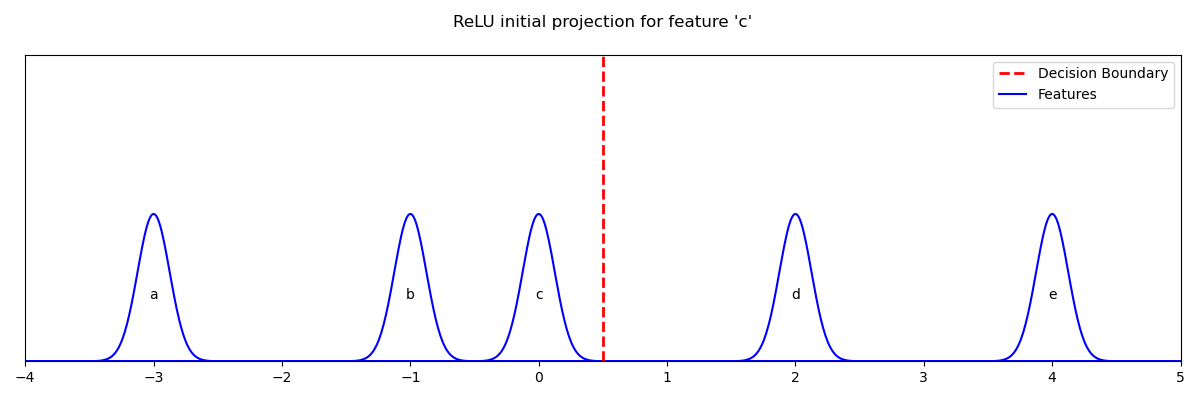
\includegraphics[width=\textwidth]{images/activation_demo_relu_pre}
    \caption{ReLU pre-activation projection}
    \label{fig:relu_pre}
    \end{subfigure}
    \hfill
    \begin{subfigure}[b]{0.49\textwidth}
    \centering
    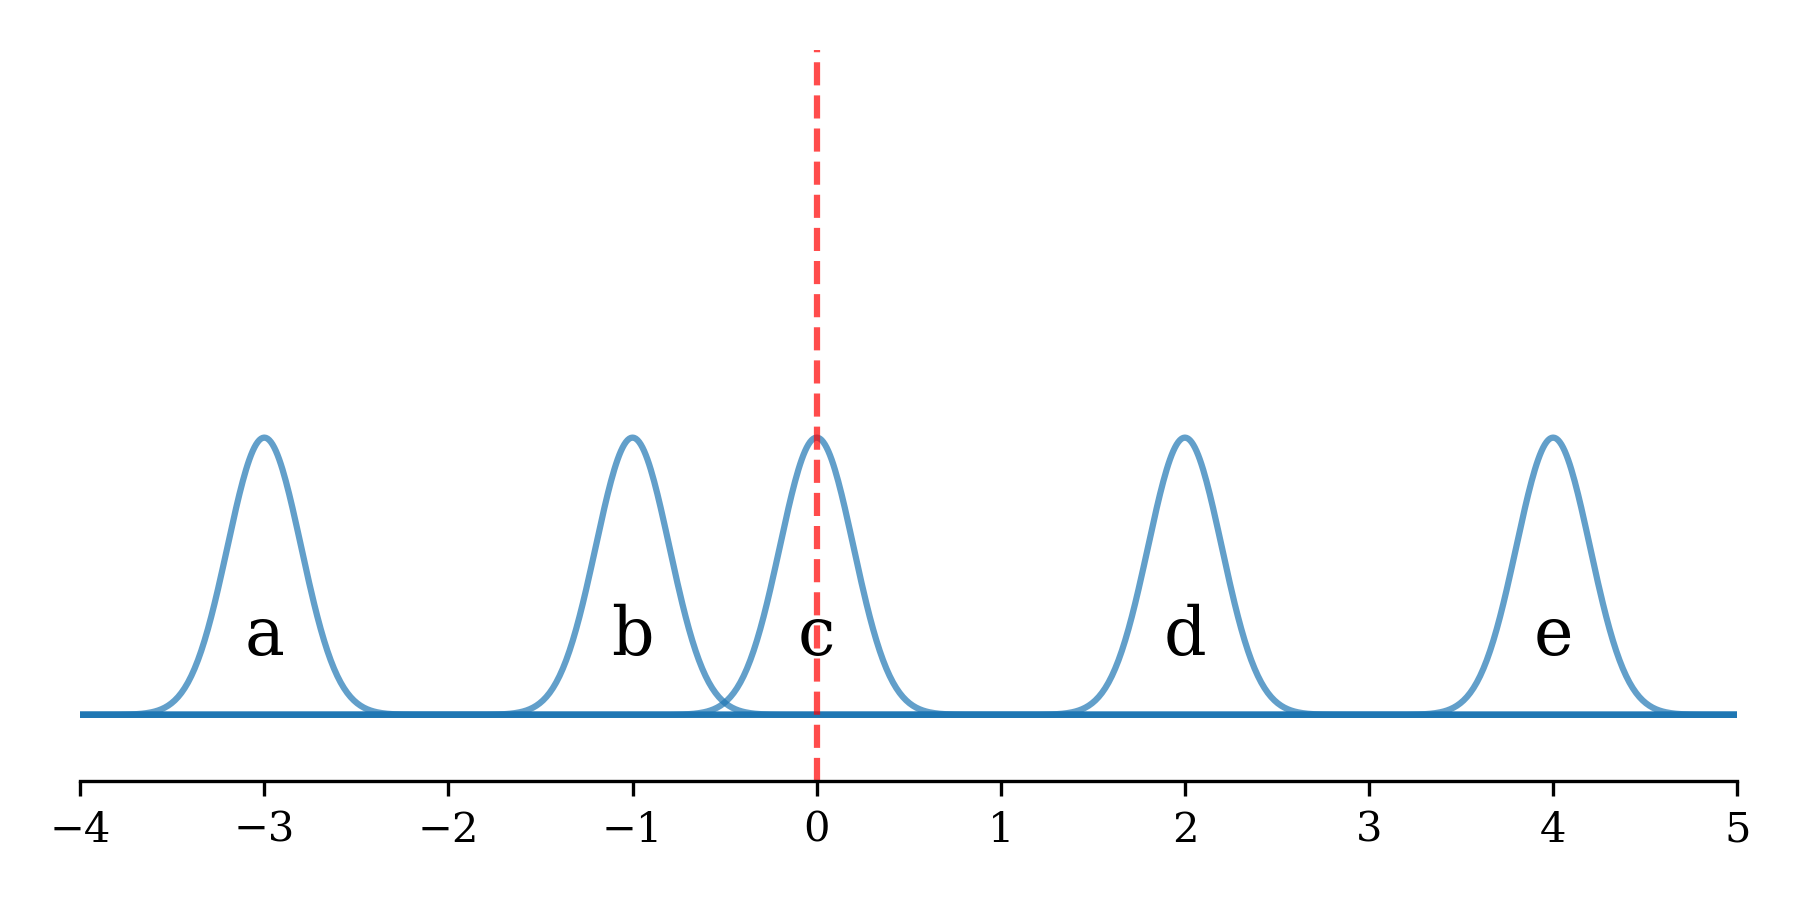
\includegraphics[width=\textwidth]{images/activation_demo_abs_pre}
    \caption{Abs pre-activation projection}
    \label{fig:abs_pre}
    \end{subfigure}

    \begin{subfigure}[b]{0.49\textwidth}
        \centering
        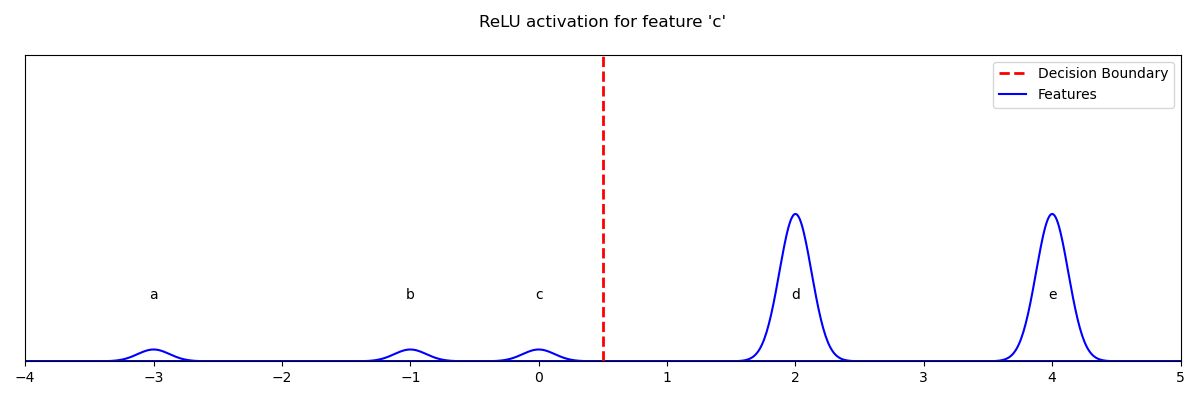
\includegraphics[width=\textwidth]{images/activation_demo_relu_post}
        \caption{ReLU post-activation response}
        \label{fig:relu_post}
    \end{subfigure}
    \hfill
    \begin{subfigure}[b]{0.49\textwidth}
        \centering
        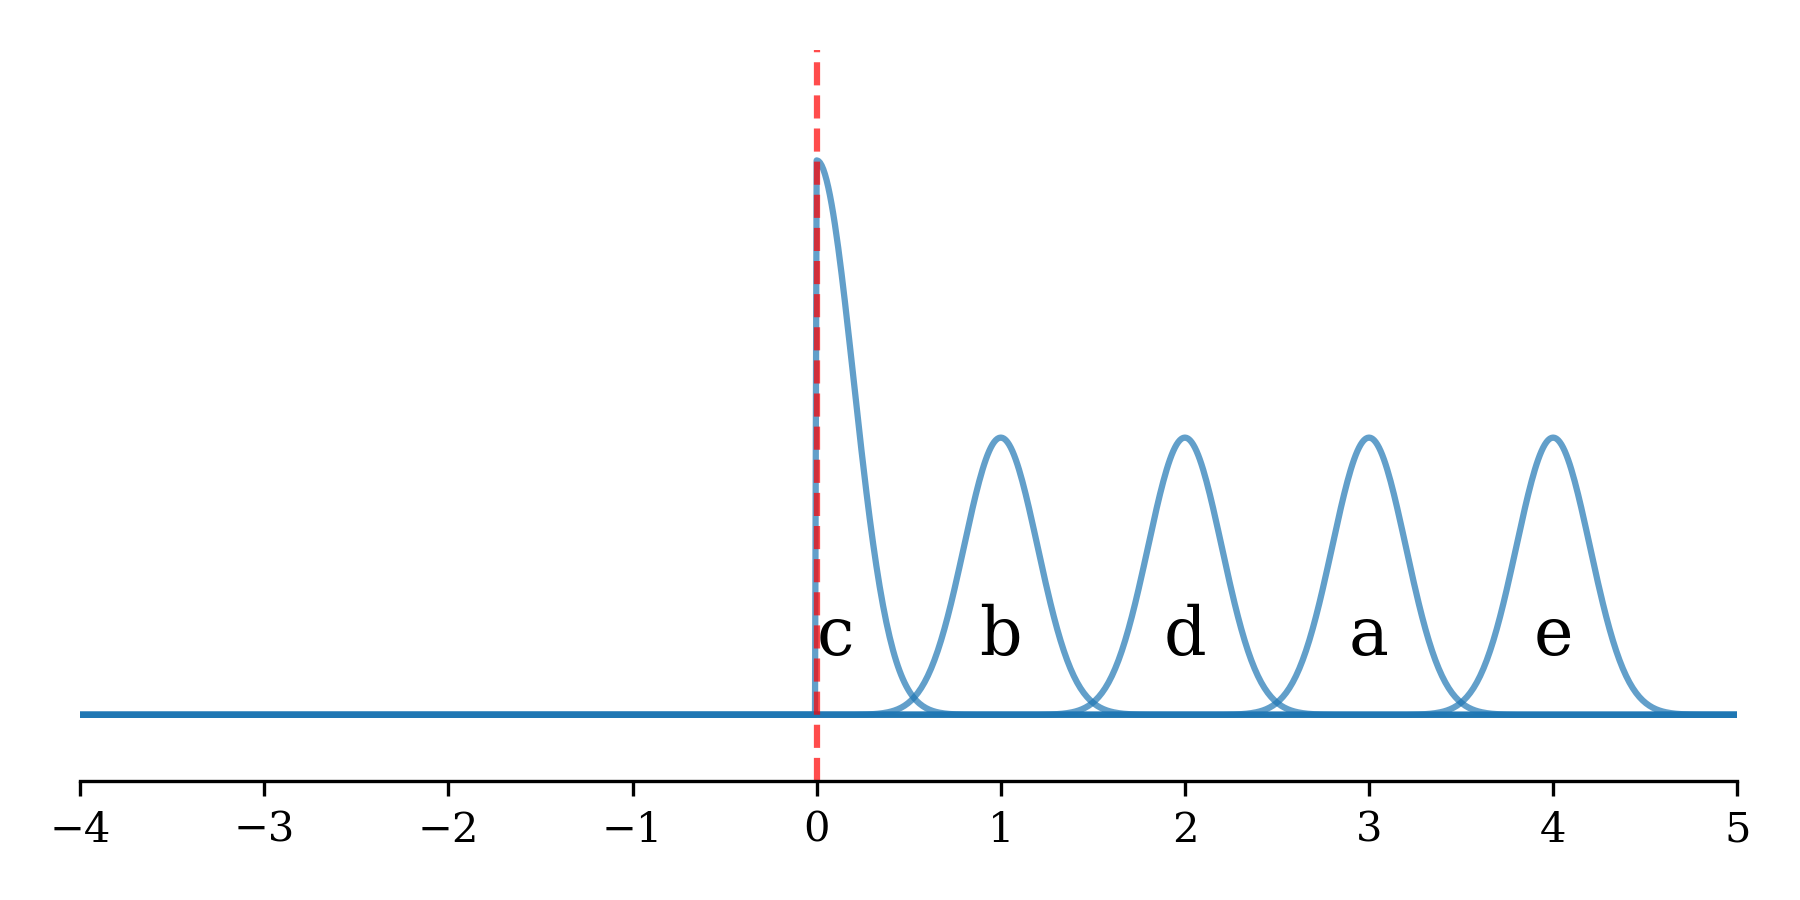
\includegraphics[width=\textwidth]{images/activation_demo_abs_post}
        \caption{Abs post-activation response}
        \label{fig:abs_post}
    \end{subfigure}

    \caption{This series of figures represents our theory on how linear nodes learn features with ReLU and Absolute Value activation functions. Each blue peak corresponds to a feature (a-e) in the hypothetical dataset, and the red dashed line denotes the decision boundary defined by the node. In the top row, the features are positioned according to their initial linear projections. The bottom row illustrates the transformed values after applying each activation function, highlighting the distinct ways that ReLU and Absolute Value modify feature space representations.}
    \label{fig:activation_demo}
\end{figure}

To aid in discussion, we explore how ReLU and Abs activations represent features within a distance metric interpretation. Figure~\ref{fig:activation_demo} illustrates the key differences in how these activation functions process information. In the pre-activation space (Figures~\ref{fig:relu_pre} and~\ref{fig:abs_pre}), both models can learn similar linear projections of input features. ReLU is driven to minimize the active feature $\left\{ c \right\}$ and ends up being positioned on the positive edge of the distribution. Abs positions the decision boundary through the mean, or possibly the median, of the data. After activation, ReLU sets all features on its dark side to the minimum possible distance: zero. Abs folds the space, moving all distributions on the negative side to the positive side. The ReLU activated node, selects for features $\left\{ a, b, c \right\}$. The folding operation of the Abs activated feature results in $\left\{ c \right\}$ being the sole feature with the smallest activation value.

\subsection{Intensity Perturbations}

\begin{figure}[t]
    \centering

    \begin{subfigure}[b]{0.49\textwidth}
        \centering
        \includegraphics[width=\textwidth]{images/tbd}
        \caption{ReLU Scaling Down 0.5x}
        \label{fig:relu_scale_down}
    \end{subfigure}
    \hfill
    \begin{subfigure}[b]{0.49\textwidth}
        \centering
        \includegraphics[width=\textwidth]{images/tbd}
        \caption{Abs Scaling Down 0.5x}
        \label{fig:relu_scale_down}
    \end{subfigure}

    \begin{subfigure}[b]{0.49\textwidth}
    \centering
    \includegraphics[width=\textwidth]{images/tbd}
    \caption{ReLU Scaling Up 2x}
    \label{fig:relu_scale_up}
    \end{subfigure}
    \hfill
    \begin{subfigure}[b]{0.49\textwidth}
    \centering
    \includegraphics[width=\textwidth]{images/tbd}
    \caption{Abs Scaling Up 2x}
    \label{fig:abs_scale_up}
    \end{subfigure}

    \caption{Effects of scaling on feature representation. The top row shows scaling down (0.5x) and the bottom row shows scaling up (2.0x) for both ReLU and Abs activated nodes.}
    \label{fig:scaling_demo}
\end{figure}

We extend our discussion with Figure~\ref{fig:scaling_demo} to demonstrate how scaling does not affect distance feature selection, but could affect intensity feature selection. All of the ReLU features are still zero. The minimum Abs feature is still the minimum. It is unclear how intensity features would be interpreted. If the following layers look for features in a band of activation values, they will find different features. CrossEntopyLoss does normalize everything at the output. If that property passes through to the hidden layer, I supposed the relative values across wouldn't change things. This needs more work. I need to see if the scale values are different for different nodes. TODO!!!

It is really difficult to explain why something that is poorly defined doesn't break.

\subsection{Offset Perturbations}

\begin{figure}[t]
    \centering

    \begin{subfigure}[b]{0.49\textwidth}
        \centering
        \includegraphics[width=\textwidth]{images/tbd}
        \caption{ReLU Offset Negative}
        \label{fig:relu_offset_down}
    \end{subfigure}
    \hfill
    \begin{subfigure}[b]{0.49\textwidth}
        \centering
        \includegraphics[width=\textwidth]{images/tbd}
        \caption{Abs Offset Negative}
        \label{fig:abs_offset_down}
    \end{subfigure}

    \begin{subfigure}[b]{0.49\textwidth}
    \centering
    \includegraphics[width=\textwidth]{images/tbd}
    \caption{ReLU Offset Positive}
    \label{fig:relu_offset_up}
    \end{subfigure}
    \hfill
    \begin{subfigure}[b]{0.49\textwidth}
    \centering
    \includegraphics[width=\textwidth]{images/tbd}
    \caption{Abs Offset Positive}
    \label{fig:abs_offset_up}
    \end{subfigure}

    \caption{Effects of decision boundary offsets on feature representation. The top row shows negative offsets  and the bottom row shows positive offsets for both ReLU and Abs activated nodes.}
    \label{fig:offset_demo}
\end{figure}

Figure~\ref{fig:offset_demo} demonstrates how offset perturbations affect feature selection. ReLU either adds or removes features to its accepted feature set. Figure a shows removes $c$ from the accept set leaving only $\left\{ a, b \right\}$. Figure c, shows ReLU accepting $\left\{ a, b, c, d \right\}$. Offset perturbations in ReLU result in incremental changes to the accept set and we can see that with the gradual performance degradation in Figure~\ref{fig:perturbation_analysis}. Abs, however, selects a single feature. Under negative offset, it shifts to select feature $\{b\}$ instead of its trained feature $\{c\}$. Under positive offset, features $\{c,d\}$ become the minimum values but neither aligns with the decision boundary and it could be interpreted as an empty set. These complete changes in feature selection explain the dramatic performance impact even with small perturbations.

The analysis of intensity features has a similar problem as the scale perturbations. TODO!!!

\subsection{The Problem with Intensity}

Our perturbation analysis appears to support distance-based feature interpretation, but we must address a significant challenge: we cannot definitively disprove intensity-based interpretations because there is no consensus on what constitutes an intensity feature. The field has proposed multiple interpretations over decades of research, yet none has emerged as definitive. Is an intensity feature indicated by maximum activation? Does it require values within a specific range? Should we consider activation values relative to other nodes? Do we need to account for normalization effects between layers?

The lack of a clear mathematical foundation for intensity metrics is particularly troubling. While distance metrics like Euclidean and Mahalanobis distances are well-defined statistical measures with clear linear formulations, we find no equivalent statistical measure for intensity that can be expressed through a linear equation. This absence is striking given the extensive study of linear methods in statistics. Without a well-defined statistical basis, intensity remains a nebulous concept, open to broad interpretations. This absence of a clear metric foundation makes it challenging to assess intensity features rigorously, raising the question of whether they are simply a subset of distance metrics in disguise.

Our scaling experiments highlight this definitional problem. If nodes measure intensity, how should scaling affect their measurements? One might expect that doubling a strong signal should make it stronger, yet our networks maintain consistent behavior under scaling. We could propose that relative values between nodes preserve the intensity information, but this begins to sound suspiciously like a distance metric in disguise.

The distance features in the network are easily explained as a Mahalanobis distance of a principal component as described in \cite{oursland2024interpreting}. But what is the statistical meaning behind the intensity features? It implies a complement to the principal component, a principal disponent consisting of an antivector, antivalue and an unmean. I don't think that principal disponents are real. What looks like an intensity metric is really a distance metric that matches everything except the large value. Perhaps statistical network interpretation has stymied researchers because we have been looking for the mathematical equivalent of Big Foot or the Loch Ness Monster.
